%-%-%-%-%-%-%-%-%-%-%-%-%-%-%-%-%-%-%-%-%-%-%-%-%-%-%-%-%-%-%-%-%-%-%-%-%-%-%
%%% MAIN DOCUMENT %%%

%-%-%-%-%-%-%-%-%-%-%-%-%-%-%-%-%-%-%-%-%-%-%-%-%-%-%-%-%-%-%-%-%-%-%-%-%-%-%

\documentclass[12pt]{article}
\usepackage{xcolor}
\usepackage{minted}

% \usepackage[T1]{fontenc}

% \usepackage{draculatheme}
% \newcommand{\documentTheme}{draculafg}
% \newcommand{\documentLogo}{../../images/small logo_white.png}
% \newcommand{\documentBigLogo}{../../images/logo_white_text.png}
% \usemintedstyle{dracula}

\newcommand{\documentBigLogo}{../../images/Hendrix Logo.png}
\newcommand{\documentLogo}{../../images/small logo.png}
\newcommand{\documentTheme}{black}

%%% AESTHETICS %%%
%-%-%-%-%-%-%-%-%-%-%-%-%-%-%-%-%-%-%-%-%-%-%-%-%-%-%-%-%-%-%-%-%-%-%-%-%-%-%


%%% Dimensions and Spacing %%%
\usepackage[margin=1in]{geometry}
\setlength{\parindent}{0pt}
\usepackage{setspace}
\usepackage{mathtools}
\usepackage{esint}
\usepackage{adjustbox}
\linespread{1}
\usepackage{listings}
\usepackage{tikz}
\usetikzlibrary{shapes,backgrounds,calc,patterns,positioning}
\usepgflibrary{shadings}
\usepackage{pgfkeys}
\usepackage{pdftexcmds}
\usepackage{shellesc}
\usepackage{algorithm, algorithmic, xspace}
\usepackage{caption}
\usepackage{subcaption}
%%% Define new colors %%%
\definecolor{orangehdx}{rgb}{0.96, 0.51, 0.16}

% Normal colors
\definecolor{xred}{HTML}{BD4242}
\definecolor{xblue}{HTML}{4268BD}
\definecolor{xgreen}{HTML}{52B256}
\definecolor{xpurple}{HTML}{7F52B2}
\definecolor{xorange}{HTML}{FD9337}
\definecolor{xdotted}{HTML}{999999}
\definecolor{xgray}{HTML}{777777}
\definecolor{xcyan}{HTML}{80F5DC}
\definecolor{xpink}{HTML}{F690EA}
\definecolor{xgrayblue}{HTML}{49B095}
\definecolor{xgraycyan}{HTML}{5AA1B9}

% Dark colors
\colorlet{xdarkred}{red!85!black}
\colorlet{xdarkblue}{xblue!85!black}
\colorlet{xdarkgreen}{xgreen!85!black}
\colorlet{xdarkpurple}{xpurple!85!black}
\colorlet{xdarkorange}{xorange!85!black}
\definecolor{xdarkcyan}{HTML}{008B8B}
\colorlet{xdarkgray}{xgray!85!black}

% Very dark colors
\colorlet{xverydarkblue}{xblue!50!black}

% Document-specific colors
\colorlet{normaltextcolor}{black}
\colorlet{figtextcolor}{xblue}

% Enumerated colors
\colorlet{xcol0}{black}
\colorlet{xcol1}{xred}
\colorlet{xcol2}{xblue}
\colorlet{xcol3}{xgreen}
\colorlet{xcol4}{xpurple}
\colorlet{xcol5}{xorange}
\colorlet{xcol6}{xcyan}
\colorlet{xcol7}{xpink!75!black}

% Blue-Purple (should just used colorbrewer...)
\definecolor{xrainbow0}{HTML}{e41a1c}
\definecolor{xrainbow1}{HTML}{a24057}
\definecolor{xrainbow2}{HTML}{606692}
\definecolor{xrainbow3}{HTML}{3a85a8}
\definecolor{xrainbow4}{HTML}{42977e}
\definecolor{xrainbow5}{HTML}{4aaa54}
\definecolor{xrainbow6}{HTML}{629363}
\definecolor{xrainbow7}{HTML}{7e6e85}
\definecolor{xrainbow8}{HTML}{9c509b}
\definecolor{xrainbow9}{HTML}{c4625d}
\definecolor{xrainbow10}{HTML}{eb751f}
\definecolor{xrainbow11}{HTML}{ff9709}

%------- %
% XHFILL %
%------- %



%%% Chapter Headings %%%

\newcommand{\gradientrule}{
    \begin{tikzpicture}
        \shade[left color=orangehdx, right color=black, middle color=gray] (0,0) rectangle (\linewidth,0.4pt);
    \end{tikzpicture}
}

\usepackage[Glenn]{fncychap}
% \ChTitleVar{\bfseries\scshape\color{\documentTheme}} % Needed for Dracula theme
% \ChNumVar{\large\selectfont\color{\documentTheme}} % Needed for Dracula theme
% \ChNameVar{\large\color{\documentTheme}} % Needed for Dracula theme
\usepackage{xpatch}

% \xpatchcmd{\DOCH}
%   {\mghrulefill}{\gradientrule\mghrulefill}
%   {}{\PatchFailed}
% \xpatchcmd{\DOTI}
%   {\mghrulefill}{\gradientrule\mghrulefill}
%   {}{\PatchFailed}
% \xpatchcmd{\DOTIS}
%   {\mghrulefill}{\gradientrule\mghrulefill}
%   {}{\PatchFailed}

\xpatchcmd\DOCH
{\mghrulefill}{\color{orangehdx}\mghrulefill}
{}{\PatchFailed}
\xpatchcmd\DOTI
{\mghrulefill}{\color{orangehdx}\mghrulefill}
{}{\PatchFailed}
\xpatchcmd\DOTIS
{\mghrulefill}{\color{orangehdx}\mghrulefill}
{}{\PatchFailed}


% \usepackage[Bjornstrup]{fncychap}

% \newcommand{\gradient}[1]{
% \begin{tikzpicture}
%     \node (rect) at (0,0) [fill=blue,,path fading=East,minimum width=\linewidth,minimum height=2.5cm] {};
%     \node(title)[above left = 10pt and 10pt of rect.south east, anchor=south east, font=\CTV] {\textcolor{horange}{#1}};
%     \ifnum \thechapter>0\node[left = 10pt of rect.north east,  anchor=center, font=\CNoV] {\textcolor{horange}{\thechapter}};\fi%
% \end{tikzpicture}%
% \vskip 40pt
% }


% \renewcommand{\DOCH}{}
% \renewcommand{\DOTI}[1]{\gradient{#1}}
% \renewcommand{\DOTIS}[1]{\gradient{#1}}

%% Change Chapter Heading Placement %%
\usepackage{etoolbox}
% \makeatletter
% \patchcmd{\@makechapterhead}{\vspace*{50\p@}}{\vspace*{-20\p@}}{}{}
% \patchcmd{\@makeschapterhead}{\vspace*{50\p@}}{\vspace*{-20\p@}}{}{}
% \patchcmd{\DOTI}{\vskip 80\p@}{\vskip 40\p@}{}{}
% \patchcmd{\DOTIS}{\vskip 40\p@}{\vskip 0\p@}{}{}
% \makeatother



% \newcommand*\chapterlabel{}\pmod
% \titleformat{\chapter}
%   {\gdef\chapterlabel{}
%    \normalfont\sffamily\Huge\bfseries\scshape}
%   {\gdef\chapterlabel{\thechapter\ }}{0pt}
%   {\begin{tikzpicture}[remember picture,overlay]
%     \node[yshift=-3cm] at (current page.north west)
%       {\begin{tikzpicture}[remember picture, overlay]
%         \draw[fill=LightSkyBlue] (0,0) rectangle
%           (\paperwidth,3cm);
%         \node[anchor=east,xshift=.9\paperwidth,rectangle,
%               sharp corners=downhill=20pt,inner sep=11pt,
%               fill=MidnightBlue]
%               {\color{white}\chapterlabel#1};
%        \end{tikzpicture}
%       };
%    \end{tikzpicture}
%   }
% \titlespacing*{\chapter}{0pt}{50pt}{-60pt}

% \usepackage[Conny]{fncychap}
% \usepackage[Rejne]{fncychap}
% \ChNameVar{\bfseries}  % Makes the chapter "Chapter #" bold
% \ChNumVar{\bfseries}   % Makes the chapter number bold
% \ChTitleVar{\bfseries} % Makes the chapter title bold
% % Define a custom color, for example:
% \definecolor{mycolor}{RGB}{0,128,255}

% % Redefine the chapter style in Rejne to change the line colors
% \makeatletter
% \ChRuleWidth{2pt}   % Change the thickness of the lines
% \renewcommand{\DOCH}{%
%   \vspace*{-50\p@}% Moves the chapter title up/down if needed
%   {\color{mycolor} \hrule \@chapapp{} \space \thechapter \hrule}% Customizes the chapter header with color
% }
% \renewcommand{\DOTI}[1]{%
%   \vskip 20\p@ % Adjusts the space above the title
%   \bfseries #1\par % Embolden the title
%   \vskip 20\p@ % Adjusts the space below the title
% }
% \makeatother

% %% Change Chapter Heading Placement %%
% \usepackage{etoolbox}
% \makeatletter
% \patchcmd{\@makechapterhead}{\vspace*{50\p@}}{\vspace*{-20\p@}}{}{}
% \patchcmd{\@makeschapterhead}{\vspace*{50\p@}}{\vspace*{-20\p@}}{}{}
% \patchcmd{\DOTI}{\vskip 80\p@}{\vskip 40\p@}{}{}
% \patchcmd{\DOTIS}{\vskip 40\p@}{\vskip 0\p@}{}{}
% \makeatother

% \renewcommand{\thesection}{\thechapter.\arabic{section}} %% Chapter.Section Numbering


%%% FIGURES %%%
\usepackage{graphicx}  
% \numberwithin{figure}{section}
\usepackage{float}
\usepackage{caption}

%%% Hyperlinks %%%
\usepackage{hyperref}
\definecolor{horange}{HTML}{f58026}
\hypersetup{
	colorlinks=true,
	linkcolor=horange,
	filecolor=horange,      
	urlcolor=horange,
}


%% Headers and Footers %%
\usepackage{fancyhdr} % This should be set AFTER setting up the page geometry
\pagestyle{fancy} % options: empty , plain , fancy
\fancyhead[R]{\assignmentname}
\fancyhead[L]{Hendrix College}
\fancyhead[C]{\includegraphics[height=.50cm]{\documentLogo}} % Use for Dracula
\usepackage{xpatch}
\xpretocmd\headrule{\color{orangehdx}}{}{\PatchFailed}
\setlength{\footskip}{0.5in}
\setlength{\headheight}{18.5764pt}


%%%%% Colored Boxes %%%%%
\usepackage{tcolorbox}
\tcbuselibrary{skins}
\tcbuselibrary{theorems}
% \tcbuselibrary{minted}
\newcounter{BoxCounter}
\usepackage{dingbat}

%-%-%-%-%-%-%-%-%-%-%-%-%-%-%-%-%-%-%-%-%-%-%-%-%-%-%-%-%-%-%-%-%-%-%-%-%-%-%

%% MATH PACKAGES, ENVIRONMENTS, COMMANDS %%
%-%-%-%-%-%-%-%-%-%-%-%-%-%-%-%-%-%-%-%-%-%-%-%-%-%-%-%-%-%-%-%-%-%-%-%-%-%-%
%You'll need your own packages, theorem types, and commands.

\usepackage{fix-cm}
\usepackage{amsmath,amsthm} 
\usepackage{array, makecell}
\usepackage{colortbl}
\newcommand{\thickvrule}{\vrule width 1pt}

\newcommand{\thickhrule}{\Xhline{1pt}}

\usepackage{mathtools}
\usepackage{amssymb}
\usepackage[framemethod=tikz]{mdframed}
\usepackage{mathrsfs}
\usepackage{changepage}
\usepackage{multicol}
\usepackage{slashed}
\usepackage{enumerate}
\usepackage{braket}
\usepackage{booktabs}
\usepackage{enumitem}
\usepackage{kantlipsum}  %This package lets us generate random text for example purposes.
\usepackage{pgfplots}


%%% Custom Commands %%%
% Natural Numbers 
\newcommand{\N}{\mathbb{N}}

% Whole Numbers
\newcommand{\W}{\mathbb{W}}

% Integers
\newcommand{\Z}{\mathbb{Z}}

% Rational Numbers
\newcommand{\Q}{\mathbb{Q}}

% Real Numbers
\newcommand{\R}{\mathbb{R}}

% Complex Numbers
\newcommand{\C}{\mathbb{C}}

\newcommand{\I}{\mathbb{I}}

\newcommand{\pfs}{\noindent\makebox[\linewidth]{\rule{\textwidth}{0.4pt}}\vspace{0.5cm}}

\newcommand{\mysqrt}[1]{%
	\mathpalette\foo{#1}%
}
\newcommand{\dmysqrt}[1]{%
	\mathpalette\foodisplay{#1}%
}

% !TeX spellcheck = off
\newcommand{\foo}[2]{%
	% #1: math style, #2: content
	\sbox0{$#1\sqrt{#2}$}% Measure the size of the standard sqrt in the current style
	\begin{tikzpicture}[baseline=(sqrt.base)]
		\node[inner sep=0, outer sep=0] (sqrt) {$#1\sqrt{#2}$}; % Use the current math style
		\draw([yshift=-0.045em]sqrt.north east) -- ++(0,-0.5ex); % Draw the tick
	\end{tikzpicture}%
}
% !TeX spellcheck = off
\newcommand{\foodisplay}[2]{%
	% #1: math style, #2: content
	\sbox0{$#1\sqrt{#2}$}% Measure the size of the standard sqrt in the current style
	\begin{tikzpicture}[baseline=(sqrt.base)]
		\node[inner sep=0, outer sep=0] (sqrt) {$\displaystyle\sqrt{#2}$}; % Force displaystyle
		\draw[line width=0.4pt] ([yshift=-0.044em]sqrt.north east) -- ++(0,-0.5ex); % Draw the tick
	\end{tikzpicture}%
}

% \renewcommand{\theenumi}{\arabic{enumi}}
% \renewcommand{\labelenumi}{\textbf{\theenumi}.}

% \newcommand{}{\marginnote{
\includegraphics[width=2em]{caution.png}}}

\newmdenv[
	topline=false,
	bottomline=true,
	rightline=false,
	leftline=true,
	linewidth=1.5pt,
	linecolor=black, % default color, will be overridden in custom commands
	% backgroundcolor=draculafg, % Needed for Dracula theme
	fontcolor=\documentTheme, % Needed for Dracula theme
	innertopmargin=0pt,
	innerbottommargin=5pt,
	innerrightmargin=10pt,
	innerleftmargin=10pt,
	leftmargin=0pt,
	rightmargin=0pt,
	skipabove=\topsep,
	skipbelow=\topsep,
]{customframedproof}

\newenvironment{proofpart}[2][black]{
    \begin{mdframed}[
        topline=false,
        bottomline=false,
        rightline=false,
        leftline=true,
        linewidth=1pt,
        linecolor=#1!40, % Custom color
        % innertopmargin=10pt,
        % innerbottommargin=10pt,
        innerleftmargin=10pt,
        innerrightmargin=10pt,
        leftmargin=0pt,
        rightmargin=0pt,
        % skipabove=\topsep,
        % skipbelow=\topsep%
    ]
    \noindent
    \begin{minipage}[t]{0.08\textwidth}%
        \textbf{#2}%
    \end{minipage}%
    \begin{minipage}[t]{0.90\textwidth}%
        \begin{adjustwidth}{0pt}{0pt}%
}{
    \end{adjustwidth}
    \end{minipage}
    \end{mdframed}
}

% Define a new environment 'proofscratch' for Proof and Scratch Paper
\newenvironment{proofscratch}[2]{%
    \begin{mdframed}[
        topline=false,
        bottomline=false,
        rightline=false,
        leftline=false,
        backgroundcolor=draculabg, % Background color for Dracula theme
        fontcolor=\documentTheme,       % Font color for Dracula theme
        innerleftmargin=-6pt,
        innertopmargin=0pt,
        leftmargin=0pt,
        rightmargin=0pt,
        skipabove=\topsep,
        skipbelow=\topsep,
    ]
    % % Begin TikZ picture for the vertical dotted line
    % \begin{tikzpicture}[overlay, remember picture]
    %     % Draw a vertical dotted line at approximately the center of the mdframed width
    %     \draw[dotted, thick] ([xshift=0.005\linewidth]current bounding box.north west) -- ([xshift=0.005\linewidth]current bounding box.south west);
    % \end{tikzpicture}%
    % % Create the left minipage for Proof
    \begin{minipage}[t]{0.47\textwidth}%
        \noindent\textit{Proof.} #1 \hfill \(\qed\)
    \end{minipage}%
    \hfill
    % Create the right minipage for Scratch Paper
    \begin{minipage}[t]{0.47\textwidth}%
        \textit{Scratch Paper.} #2
    \end{minipage}%
}{
    \end{mdframed}
}

\newenvironment{tipbox}
	{%
		\par\noindent%
		% Top dashed line (using \textwidth)
		\tikz[baseline]{\draw[dash pattern=on 3pt off 2pt, line width=0.5pt, color=draculapurple] (0,0) -- (\textwidth,0);}%
		\par\vspace{0.65em}%
		\noindent\textbf{\textcolor{draculapurple}{TIP:}}\quad%
	}
	{%
		\par%
		% Bottom dashed line
		\noindent%
		\tikz[baseline]{\draw[dash pattern=on 3pt off 2pt, line width=0.5pt, color=draculapurple] (0,0) -- (\textwidth,0);}%
		\par\vspace{0.35em}
	}

\newenvironment{notebox}
	{%
		\par\noindent%
		% Top dashed line (using \textwidth)
		\tikz[baseline]{\draw[dash pattern=on 3pt off 2pt, line width=0.5pt, color=draculagreen] (0,0) -- (\textwidth,0);}%
		\par\vspace{0.65em}%
		\noindent\textbf{\textcolor{draculagreen}{NOTE:}}\quad%
	}
	{%
		\par%
		% Bottom dashed line
		\noindent%
		\tikz[baseline]{\draw[dash pattern=on 3pt off 2pt, line width=0.5pt, color=draculagreen] (0,0) -- (\textwidth,0);}%
		\par\vspace{0.35em}
	}

\newenvironment{warningbox}
	{%
		\par\noindent%
		% Top dashed line (using \textwidth)
		\tikz[baseline]{\draw[dash pattern=on 3pt off 2pt, line width=0.5pt, color=draculared] (0,0) -- (\textwidth,0);}%
		\par\vspace{0.65em}%
		\noindent\textbf{\textcolor{draculared}{WARNING:}}\quad%
	}
	{%
		\par%
		% Bottom dashed line
		\noindent%
		\tikz[baseline]{\draw[dash pattern=on 3pt off 2pt, line width=0.5pt, color=draculared] (0,0) -- (\textwidth,0);}%
		\par\vspace{0.35em}
	}

\newenvironment{solution}{\textit{Solution.}}

\newcommand{\sol}[1]{
    \begin{customframedproof}[linecolor=orangehdx!75,]
        \begin{solution}
        #1
        \end{solution}
    \end{customframedproof}
}

\newcommand{\pf}[1]{
    \begin{customframedproof}[linecolor=orangehdx!75]
        \begin{proof}
        #1
        \end{proof}
    \end{customframedproof}
}

\def \proofDistance {10pt}

\newcommand{\disabs}[1]{\ensuremath{\left|#1\right|}}
\newcommand{\limn}{\lim_{n \rightarrow \infty}}
\newcommand{\limx}[2]{\lim_{x \rightarrow #1}#2}

\newcommand{\limc}[1]{\lim_{x \rightarrow c}#1}

\newcommand{\ninn}{n \in \N}

\newcommand{\mb}[1]{\mathbf{#1}}

\newcommand{\limsupn}[1]{\limsup_{n\rightarrow \infty}#1}
\newcommand{\liminfn}[1]{\liminf_{n\rightarrow \infty}#1}


\newcommand{\proj}{\text{proj}}

\newcommand{\p}{\partial}

\newcommand{\dydx}{\frac{dy}{dx}}
\newcommand{\dxdy}{\frac{dx}{dy}}
\newcommand{\dydt}{\frac{dy}{dt}}
\newcommand{\dxdt}{\frac{dx}{dt}}
\newcommand{\dzdt}{\frac{dz}{dt}}

\newcommand{\barNotationT}[1]{\bigg|_{t = #1}}

\newcommand{\cyanit}[1]{\textit{\textcolor{cyan}{#1}}}

\newcommand{\brackett}[1]{\left\langle #1 \right\rangle}

\newcommand{\norm}[1]{\left\lVert \mathbf{#1}\right\rVert}

\newcommand{\imb}{\mb{i}}
\newcommand{\jmb}{\mb{j}}
\newcommand{\kmb}{\mb{k}}
\newcommand{\rmb}{\mb{r}}
\newcommand{\umb}{\mb{u}}

\newcommand{\vecfuc}[2]{\mb{#1}(#2)}
\newcommand{\dvecfuc}[2]{\mb{#1}'(#2)}
\newcommand{\normdvecfuc}[2]{\|\mb{#1}'(#2)\|}

\newcommand{\squigglyline}{%
    \noindent
    \tikz[baseline=-0.5ex]{
        \draw[decorate, decoration={snake, amplitude=0.5mm, segment length=3mm}] 
        (0,0) -- (\dimexpr\linewidth\relax,0);
    }%
}


% end of preamble
%-%-%-%-%-%-%-%-%-%-%-%-%-%-%-%-%-%-%-%-%-%-%-%-%-%-%-%-%-%-%-%-%-%-%-%-%-%-%

\begin{document}

\numberwithin{BoxCounter}{section}


%-%-%-%-%-%-%-%-%-%-%-%-%-%-%-%-%-%-%-%-%-%-%-%-%-%-%-%-%-%-%-%-%-%-%-%-%-%-%
%%% COVER PAGE %%%
%-%-%-%-%-%-%-%-%-%-%-%-%-%-%-%-%-%-%-%-%-%-%-%-%-%-%-%-%-%-%-%-%-%-%-%-%-%-%

\newcommand{\assignmentname}{Writing Assignment 1: Distributions}

% Do not use all caps.
\newcommand{\cussubtitle}{Probability and Statistics}
% Date format should be like: "January 1, 2001"
\newcommand{\finaldate}{September 17, 2025}
% Be sure to include degree recognition (e.g., B.S., M.S., Ph.D)
\newcommand{\professor}{Prof.\ Lars Seme, M.S.}

%-%-%-%-%-%-%-%-%-%-%-%-%-%-%-%-%-%-%-%-%-%-%-%-%-%-%-%-%-%-%-%-%-%-%-%-%-%-%

\begin{titlepage}
    \begin{center}

        \vspace*{-2cm}
        \includegraphics[width=0.8\textwidth]{\documentBigLogo}\\
        \vfill

        % Horizontal line above the title in 'horange' color
        \textcolor{horange}{\rule{\textwidth}{1.0pt}}

        \vspace{2em}

        {\huge \textbf{\assignmentname}}

        \vspace{1em} % Space between the title and the bottom line

        \textcolor{horange}{\rule{\textwidth}{1.0pt}}

        \vspace*{1\baselineskip}

        {\LARGE \textbf{\cussubtitle}}

        \begin{large}
            \vspace*{5\baselineskip}

            \vspace*{1\baselineskip}

            \emph{Author} \\[1ex]
            %Submitted by \\[\baselineskip]
            {\Large Paul Beggs \\ \par} % Editor list
            {\href{mailto:BeggsPA@Hendrix.edu}{{BeggsPA@Hendrix.edu}}}\\ % Editor affiliation

            \vspace*{1\baselineskip}

            \textit{Instructor} \\[1ex] % Tagline(s) or further description
            \professor

            \vspace*{1\baselineskip}

            \textit{Due}\\[1ex]
            {\scshape  \finaldate} \\[0.3\baselineskip] % Year published

            \thispagestyle{empty}

        \end{large}
    \end{center}
\end{titlepage}

\section{Introduction}

Probability and statistics rely on the concept of a distribution, which describes how the values of a random variable are spread across possible outcomes. Understanding a distribution's characteristics and properties are key to interpret data. Therein, the goal of this paper is to look into the relationship between relative frequency and the probability distribution function (pdf), the connection between cumulative frequency and the cumulative distribution function (cdf), and to explore five different distributions to investigate their properties.

\section{Relative Frequency \& the PDF}

The relative frequency of a value in a dataset is the number of times that value occurs divided by the total number of observations. Similarly, the pdf describes the likelihood of each possible outcome of a random variable. Thus, when we plot the relative frequency against the values of \(x\), we are essentially visualizing the pdf of the distribution.

\section{Cumulative Frequency \& the CDF}

In a similar fashion, when we measure the cumulative frequency, we are looking at the total number of observations that fall below or at a certain value of \(x\). So, when we take the cumulative frequency and plot it against \(x\), we are visualizing the cdf of the distribution. We can utilize the cdf to look at an entire distribution at once, rather than just individual points.

\section{Analysis of Distributions A through E}

The following figures illustrate the relative frequency and cumulative frequency for each of the five distributions, A through E. Each distribution is represented by two graphs: one for the relative frequency (pdf) and one for the cumulative frequency (cdf). Each distribution contains 100 data points, with each point having an associated frequency. Because of this setup, we can find important statistics such as the mean, median, mode, variance, and intervals that contain the middle 50\% and 90\% frequency intervals of the data. These are presented in the Results section. \\

To find the statistics that we are after for each distribution, we heavily rely upon the relative and cumulative frequency data. That is, for the mean, we multiply each value of \(x\) by its relative frequency and sum the results. For the median, we look for the value of \(x\) where the cumulative frequency reaches 50\%. The mode is determined by identifying the value of \(x\) with the highest relative frequency. The variance is calculated by finding the average of the squared differences from the mean, weighted by the relative frequencies. Finally, to find the intervals that contain the middle 50\% and 90\% of the data, we look for the values of \(x\) that correspond to cumulative frequencies of 25\% and 75\% for the 50\% interval, and 5\% and 95\% for the 90\% interval.  

\subsection{Comparing Distributions}

Each distribution had different corresponding frequencies for each value of \(x\). This led to different shapes and characteristics for each distribution. For example, \hyperref[fig:distA]{Distribution A} had consisted only of values 1 and 0, so the most frequently appearing value was 1, hence the mode was a range of \(x\)-values associated with a 1 in the distribution. On the other hand, \hyperref[fig:distE]{Distribution E} had a very tight clustering of values around 4, leading to a very small variance of 0.2. This distribution also had a normal shape, with the mean, median, and mode all being equal to 4.0. In contrast, \hyperref[fig:distC]{Distribution C} had a wider spread of values, evidenced with a high variance of 7.8. Additionally, this distribution had a tail that was similar to \hyperref[fig:distB]{Distribution B}, but included a spike of values around 9.0.


\section{Results}

\begin{multicols}{2}
    \begin{itemize}
        \item \hyperref[fig:distA]{\textbf{Distribution A}}
        \begin{itemize}
            \item Mean: 4.1
            \item Median: 3.9
            \item Mode: [0.1, 8.0]
            \item Variance: \(5.3\)
            \item 50\% Interval: [2.0, 6.0]
            \item 90\% Interval: [0.4, 7.6]
        \end{itemize}
        \item \hyperref[fig:distB]{\textbf{Distribution B}}
        \begin{itemize}
            \item Mean: 4.0
            \item Median: 3.5
            \item Mode: 0.1
            \item Variance: 7.7
            \item 50\% Interval: [1.6, 6.1]
            \item 90\% Interval: [0.3, 9.1]
        \end{itemize}
        \item \hyperref[fig:distC]{\textbf{Distribution C}}
        \begin{itemize}
            \item Mean: 4.0
            \item Median: 3.4
            \item Mode: 0.1
            \item Variance: 7.8
            \item 50\% Interval: [1.5, 5.9]
            \item 90\% Interval: [0.3, 9.0]
        \end{itemize}
        \item \hyperref[fig:distD]{\textbf{Distribution D}}
        \begin{itemize}
            \item Mean: 4.0
            \item Median: 3.9
            \item Mode: 3.8
            \item Variance: 4.1
            \item 50\% Interval: [2.4, 5.3]
            \item 90\% Interval: [0.8, 7.5]
        \end{itemize}
        \item \hyperref[fig:distE]{\textbf{Distribution E}}
        \begin{itemize}
            \item Mean: 4.0
            \item Median: 4.0
            \item Mode: 4.0
            \item Variance: 0.2
            \item 50\% Interval: [3.7, 4.2]
            \item 90\% Interval: [3.3, 4.6]
        \end{itemize}
        \item[\(\phantom{bullet}\)] \(\phantom{\textbf{Distribution E}}\)
        \begin{itemize}[label=\(\phantom{\bullet}\)]
            \item \(\phantom{Mean: 4.0}\)
            \item \(\phantom{Median: 4.0}\)
            \item \(\phantom{Mode: 4.0}\)
            \item \(\phantom{2}\)
            \item \(\phantom{3}\)
            \item \(\phantom{3}\)
        \end{itemize}
    \end{itemize}
\end{multicols}


\newpage

\section{Conclusion}

Through this investigation of distributions and their properties, we have found that by calculating the relative frequency and cumulative frequency, and plot them against \(x\), we can visualize the pdf and cdf of a distribution. This allows us to extract statistics such as the mean, median, mode, variance, and intervals that contain the middle 50\% and 90\% of the data. Each distribution had its own unique characteristics, which were reflected in these statistics. In some cases (such as \hyperref[fig:distC]{Distribution C}), the mean, median, and mode did not inform us about the spike around 9.0, which was only visible when looking at the graphs. This highlights the importance of visualizing data in addition to calculating summary statistics, as it can reveal patterns and features that may not be immediately apparent from the numbers alone.

\section{Graphs of Distributions A through E}

\begin{figure}[h!]
    \centering
    \begin{subfigure}[b]{0.45\textwidth}
        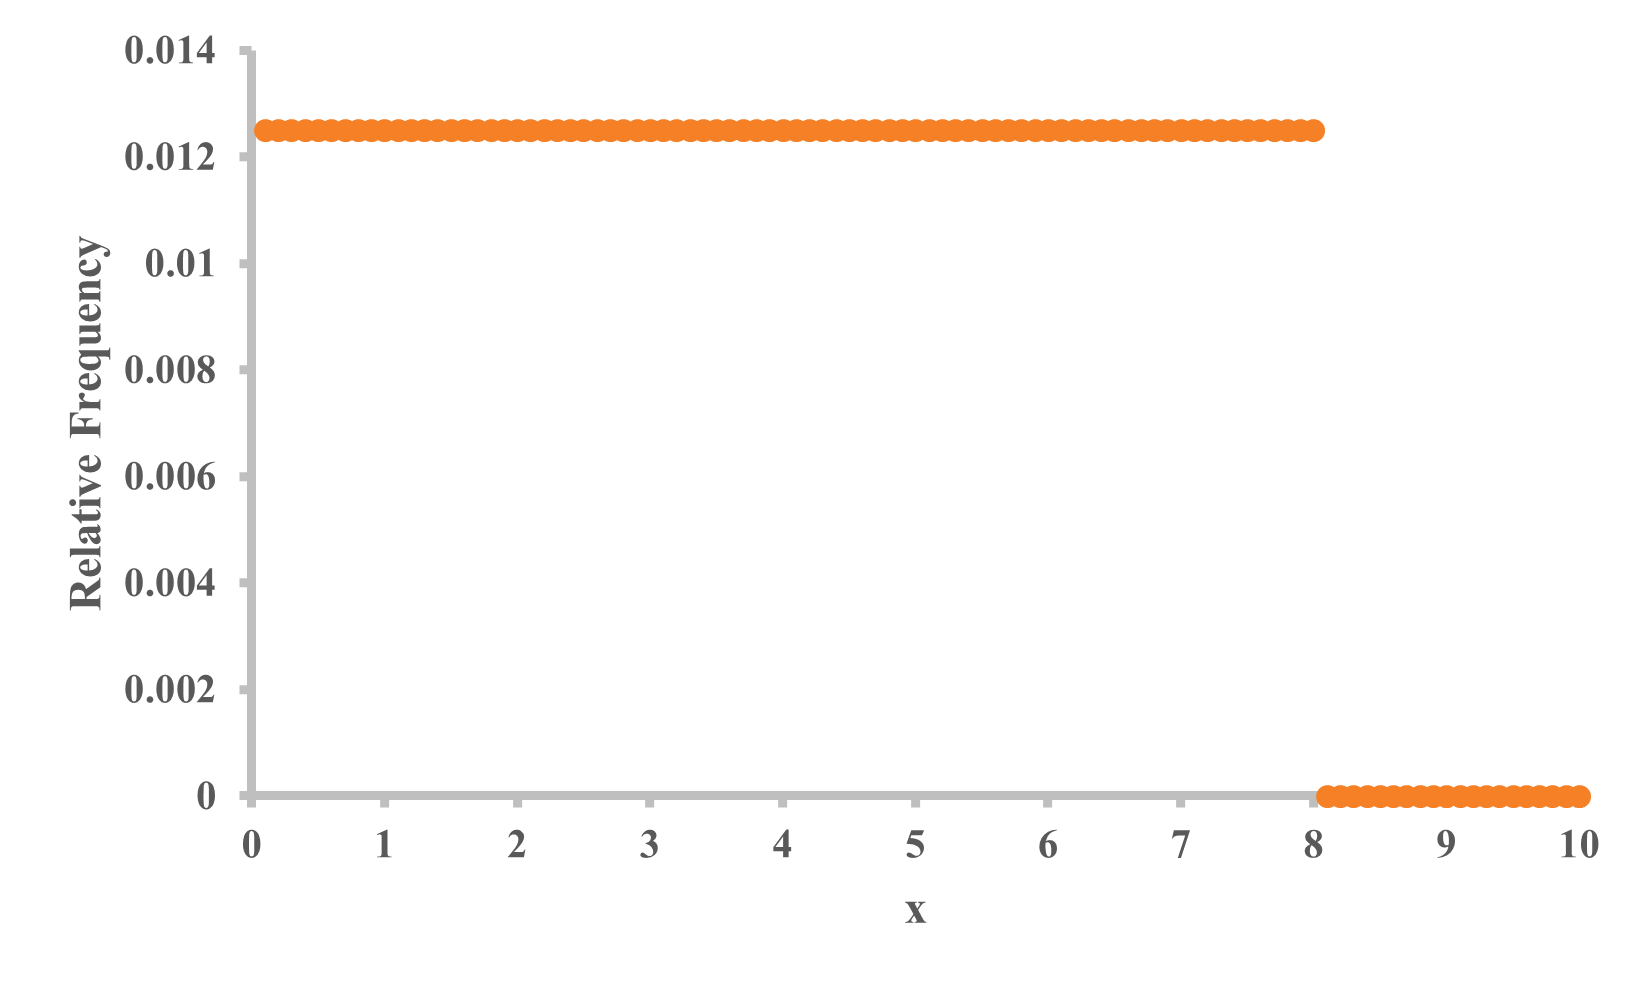
\includegraphics[width=\textwidth]{graphs/DistA_Rel.png}
        \caption{Relative Frequency vs.\ \(x\)}
    \end{subfigure}
    \hfill
    \begin{subfigure}[b]{0.45\textwidth}
        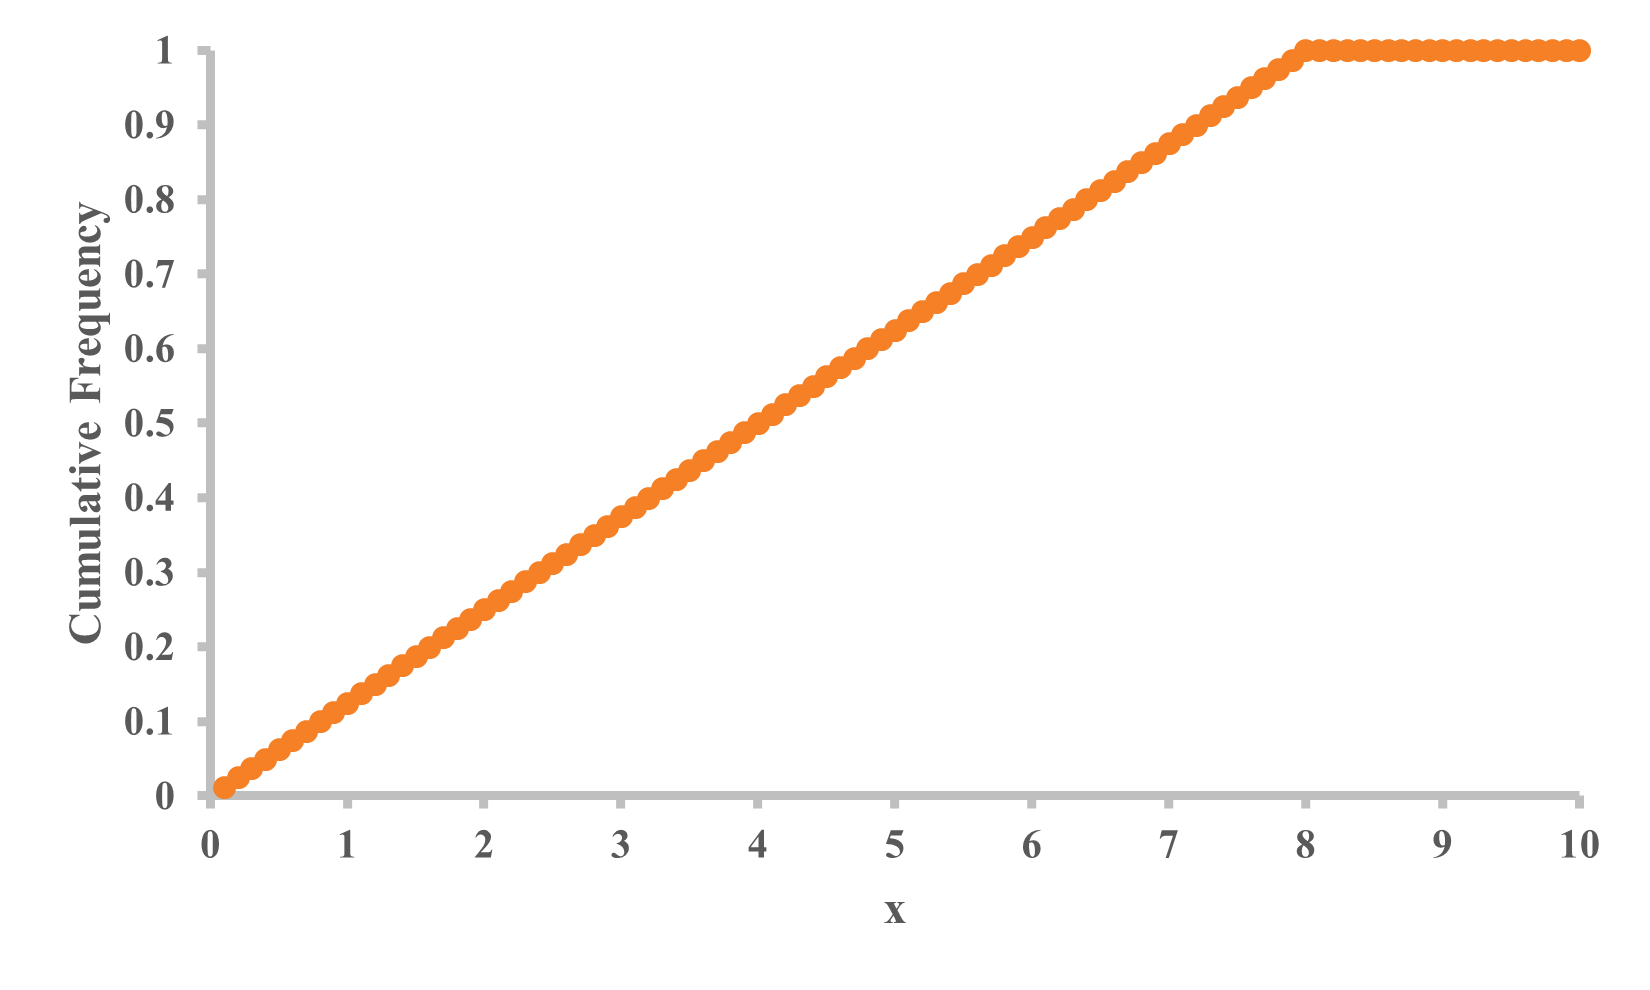
\includegraphics[width=\textwidth]{graphs/DistA_Cumul.png}
        \caption{Cumulative Frequency vs.\ \(x\)}
    \end{subfigure}
    \label{fig:distA}
    \caption{Distribution A}
\end{figure}

\begin{figure}[h!]
    \centering
    \begin{subfigure}[b]{0.45\textwidth}
        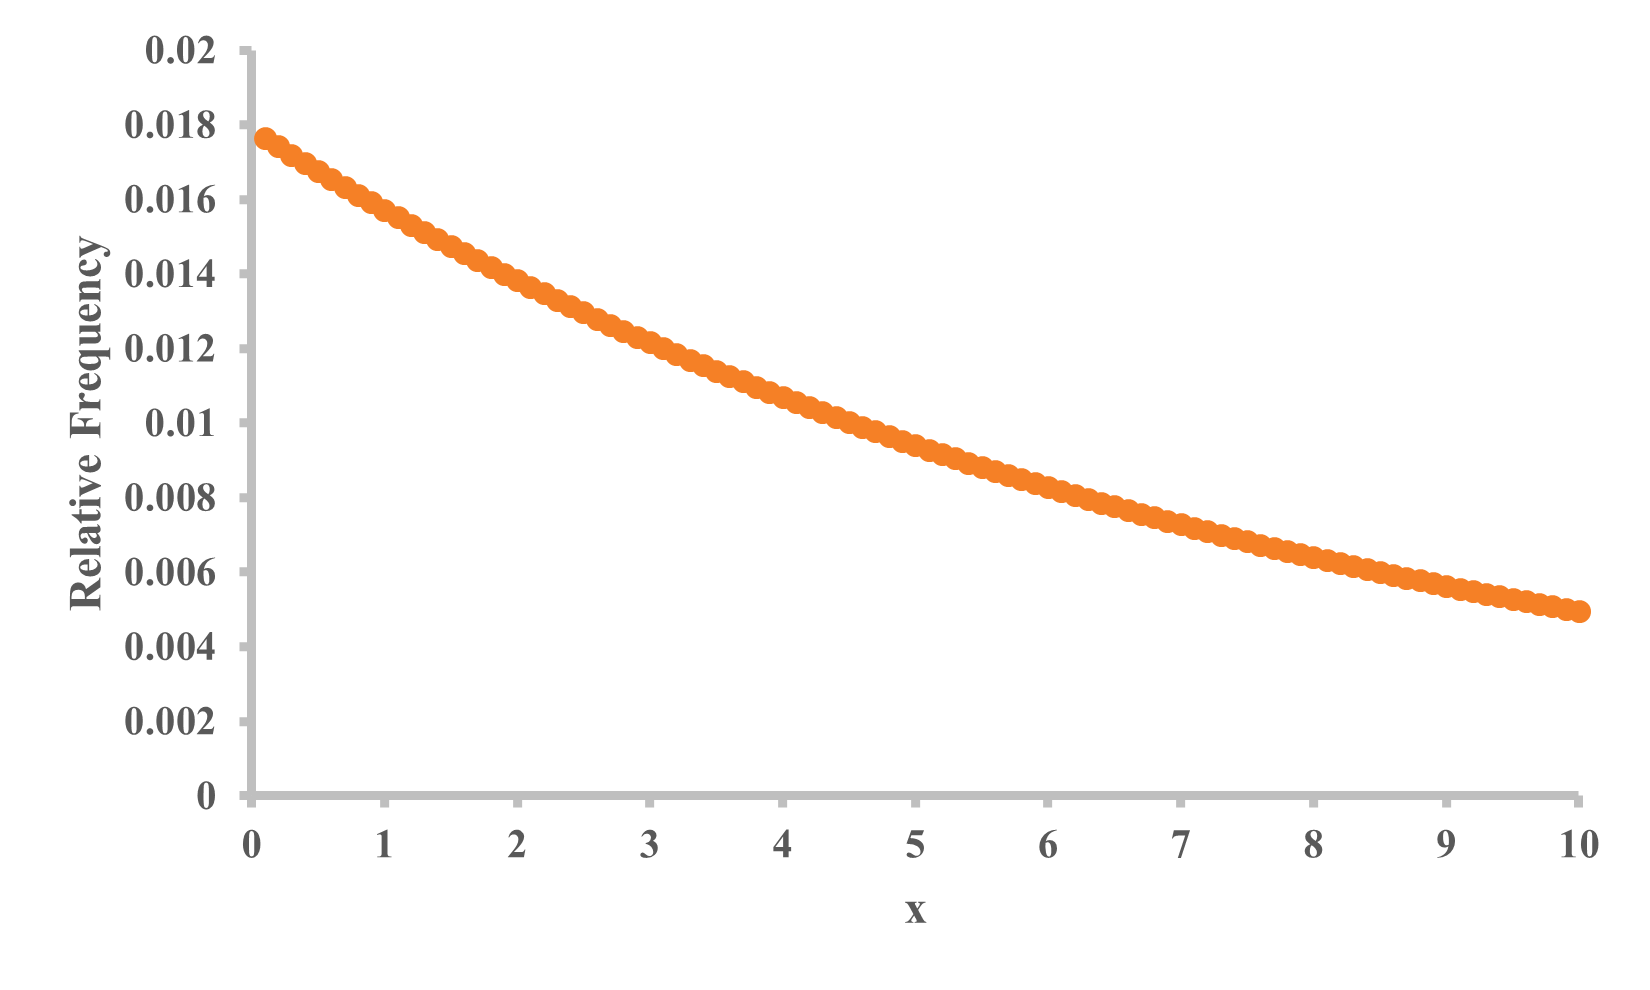
\includegraphics[width=\textwidth]{graphs/DistB_Rel.png}
        \caption{Relative Frequency vs.\ \(x\)}
    \end{subfigure}
    \hfill
    \begin{subfigure}[b]{0.45\textwidth}
        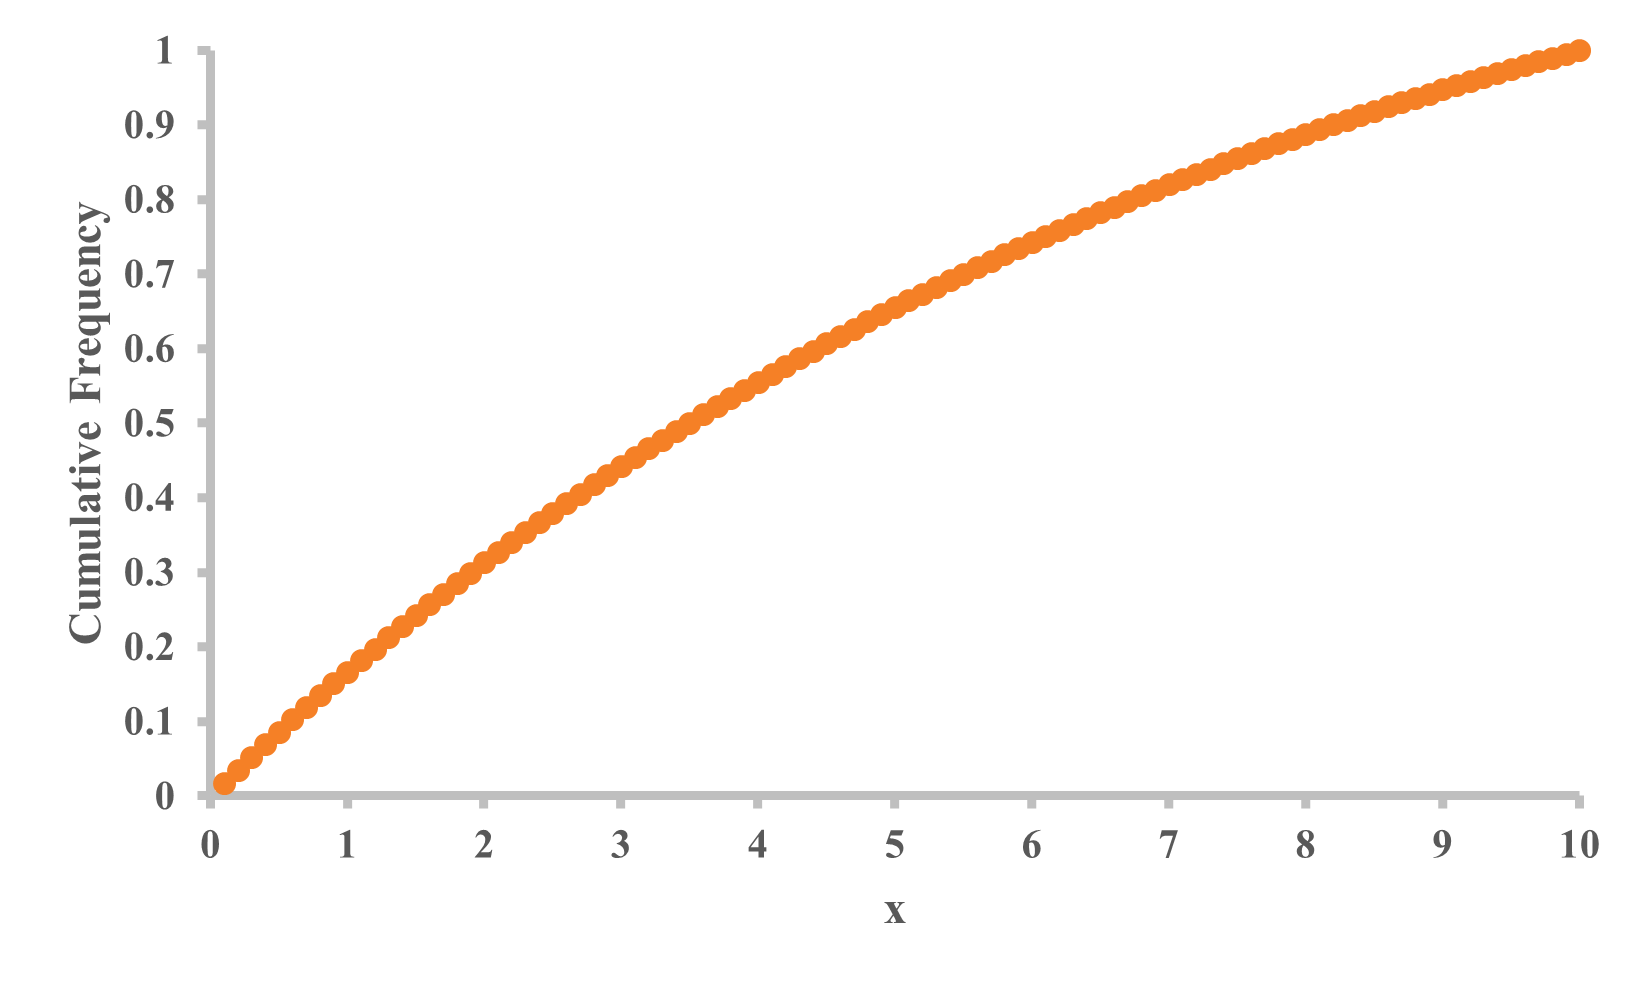
\includegraphics[width=\textwidth]{graphs/DistB_Cumul.png}
        \caption{Cumulative Frequency vs.\ \(x\)}
    \end{subfigure}
    \label{fig:distB}
    \caption{Distribution B}
\end{figure}

\begin{figure}[h!]
    \centering
    \begin{subfigure}[b]{0.45\textwidth}
        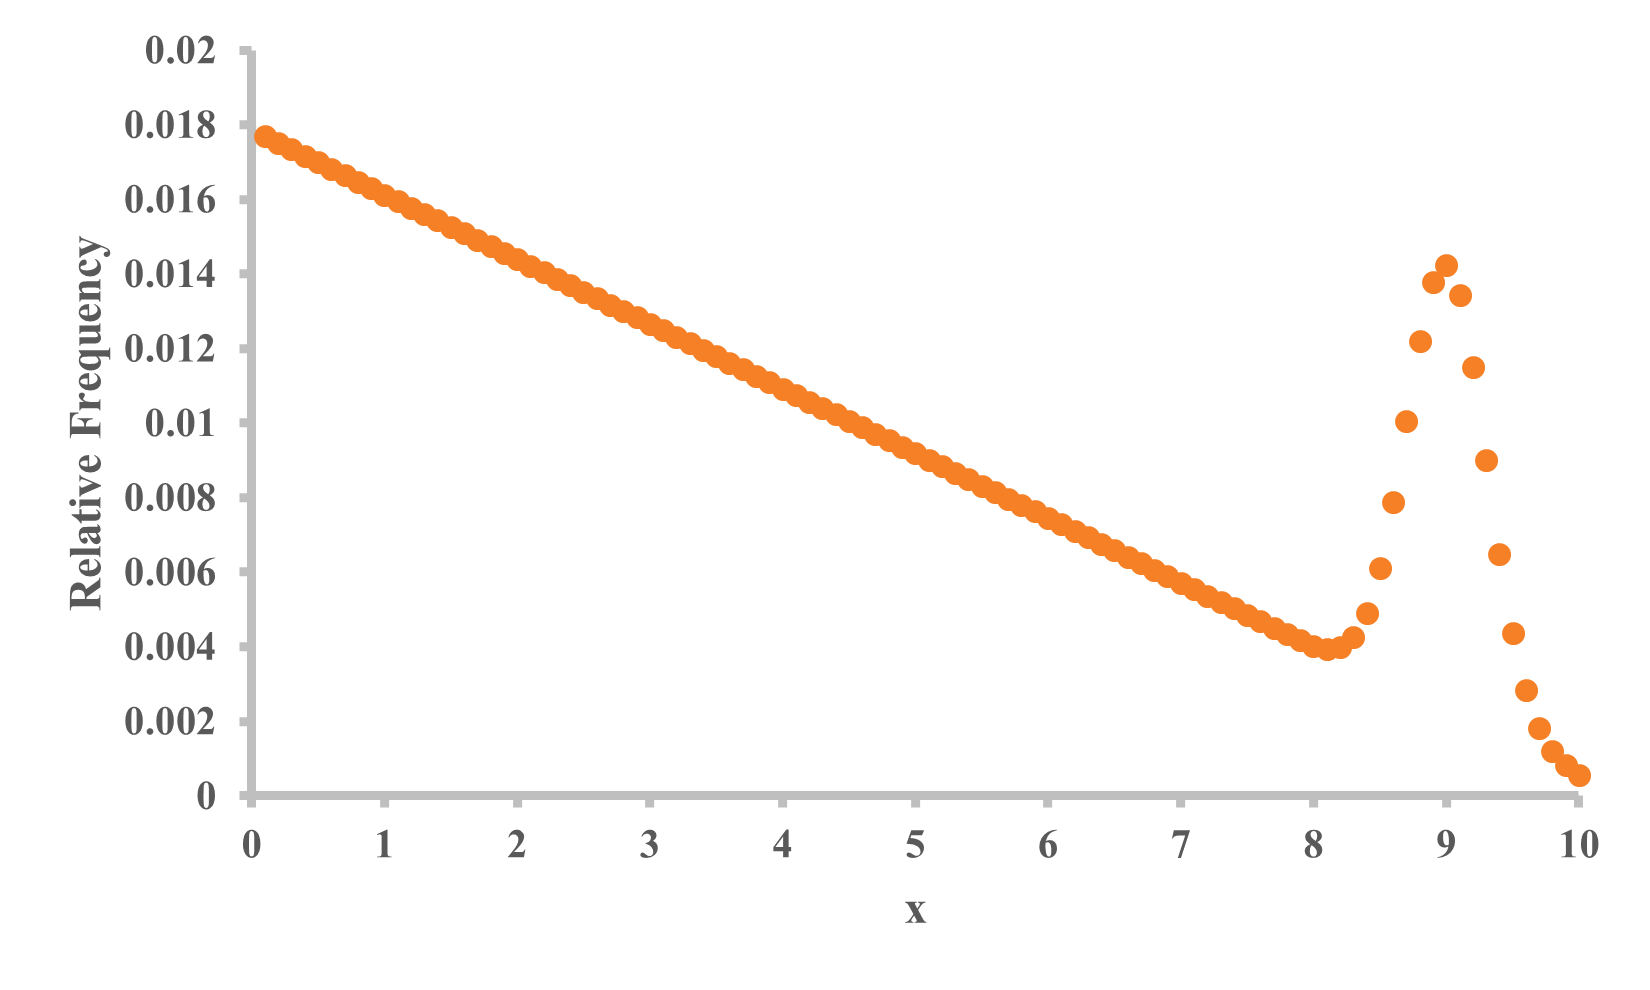
\includegraphics[width=\textwidth]{graphs/DistC_Rel.png}
        \caption{Relative Frequency vs.\ \(x\)}
    \end{subfigure}
    \hfill
    \begin{subfigure}[b]{0.45\textwidth}
        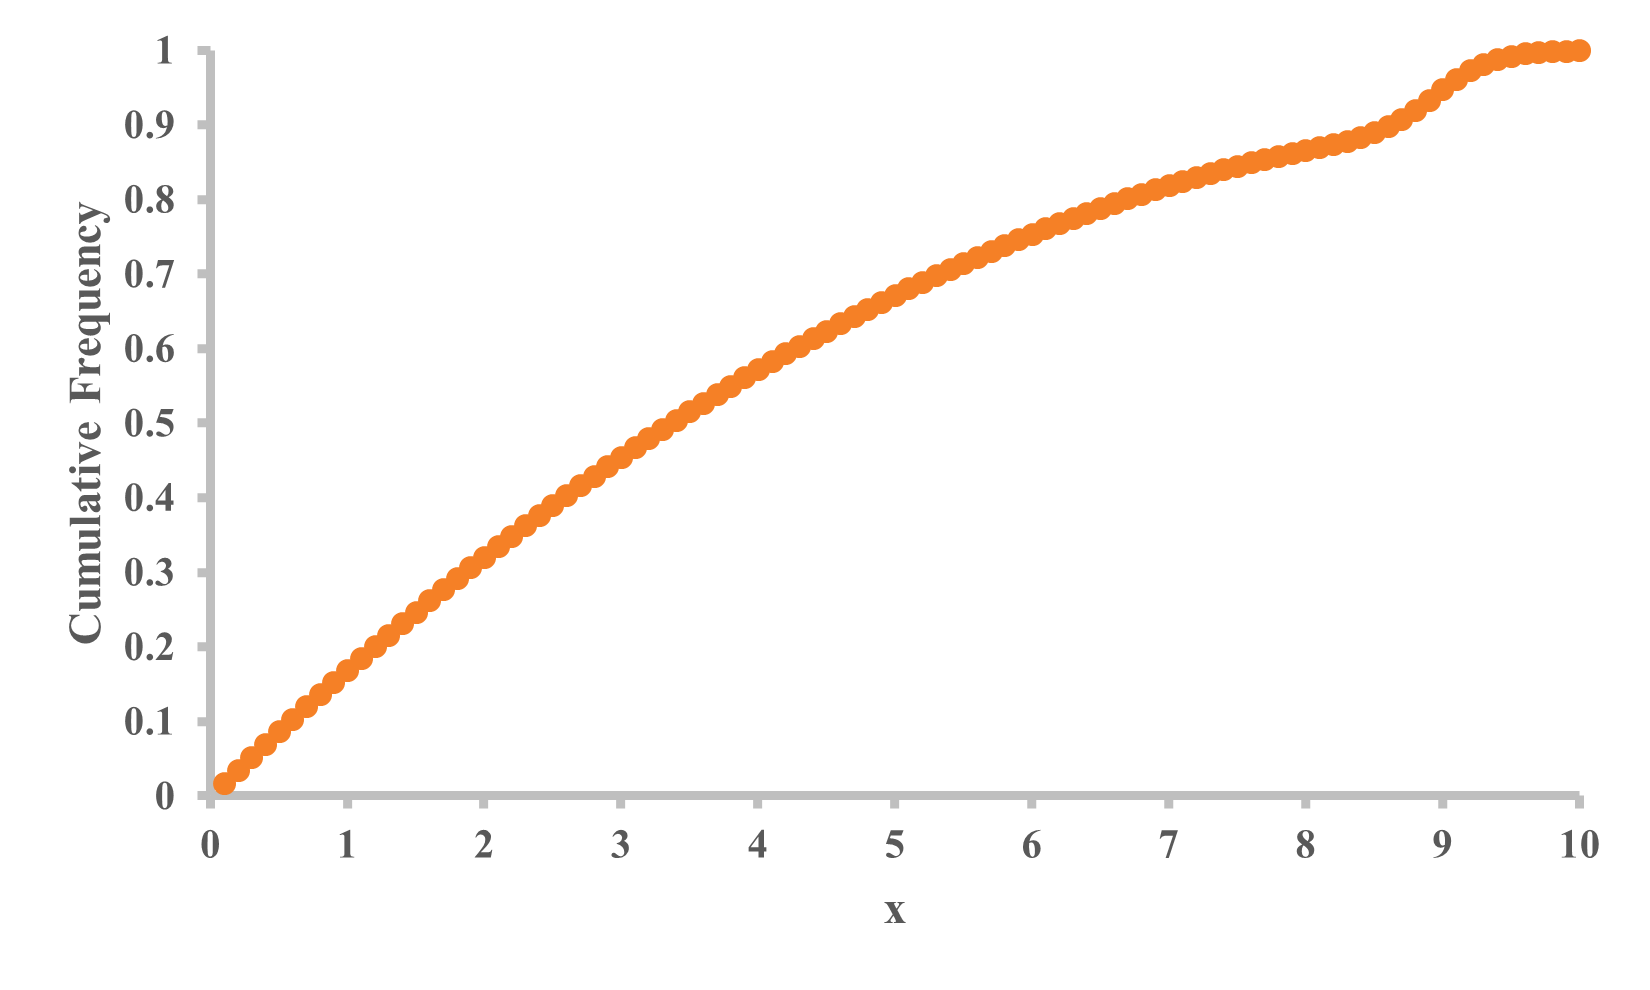
\includegraphics[width=\textwidth]{graphs/DistC_Cumul.png}
        \caption{Cumulative Frequency vs.\ \(x\)}
    \end{subfigure}
    \label{fig:distC}
    \caption{Distribution C}
\end{figure}

\begin{figure}[h!]
    \centering
    \begin{subfigure}[b]{0.45\textwidth}
        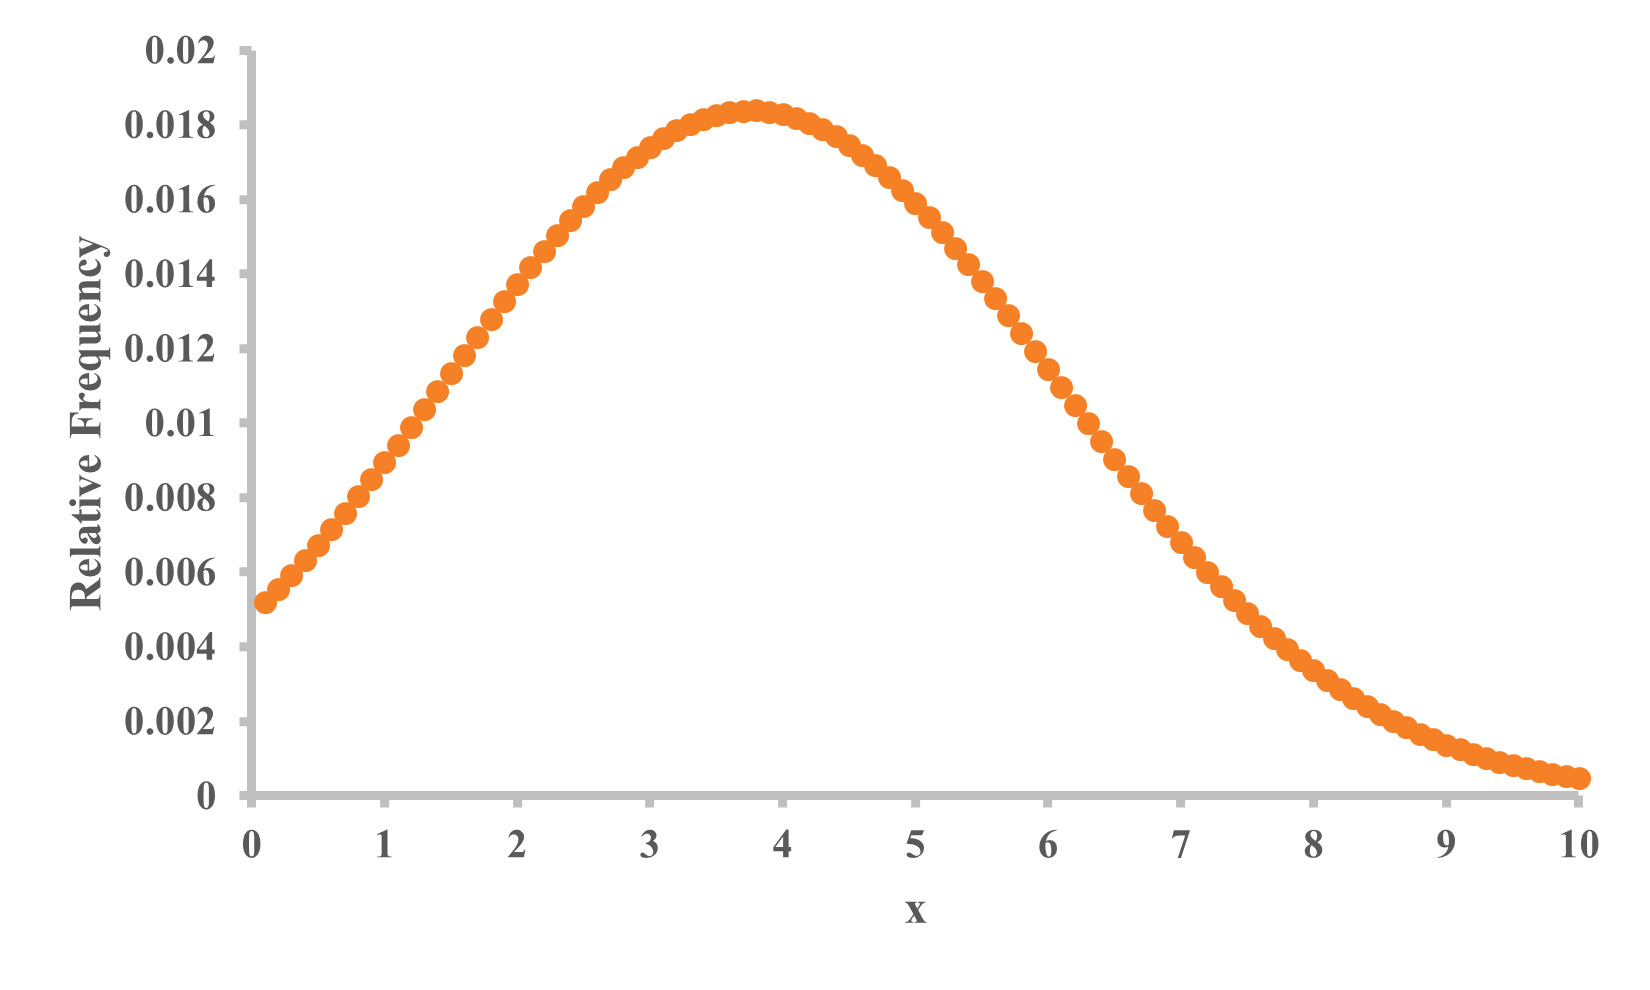
\includegraphics[width=\textwidth]{graphs/DistD_Rel.png}
        \caption{Relative Frequency vs.\ \(x\)}
    \end{subfigure}
    \hfill
    \begin{subfigure}[b]{0.45\textwidth}
        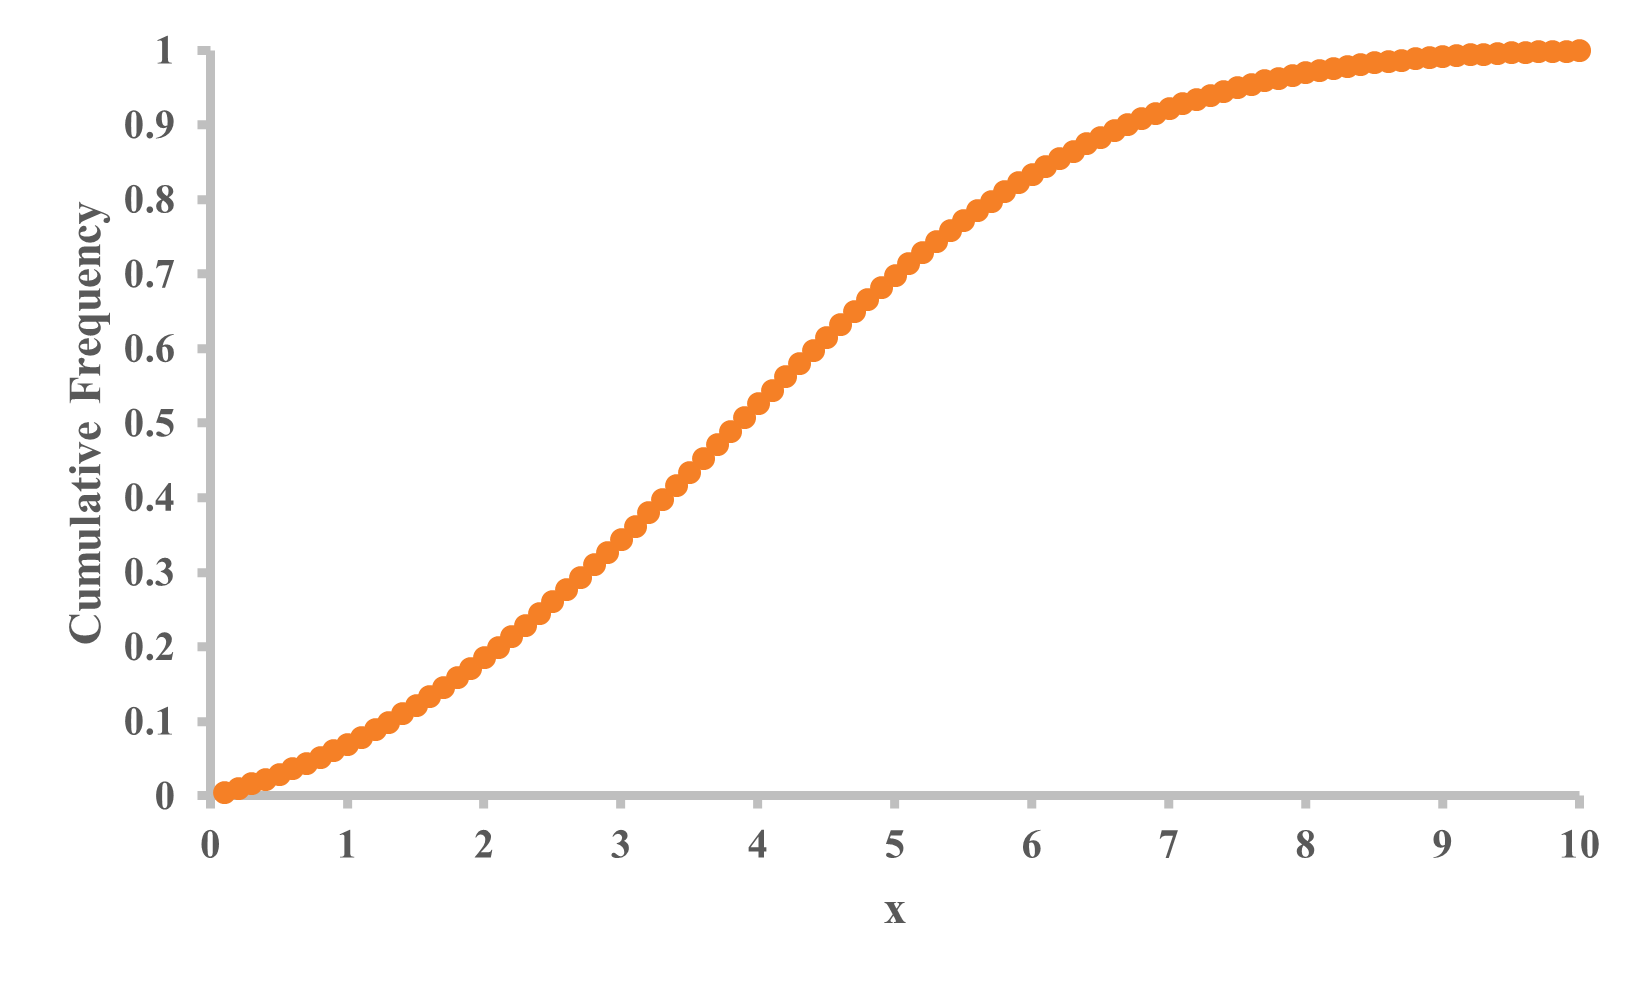
\includegraphics[width=\textwidth]{graphs/DistD_Cumul.png}
        \caption{Cumulative Frequency vs.\ \(x\)}
    \end{subfigure}
    \label{fig:distD}
    \caption{Distribution D}
\end{figure}

\begin{figure}[h!]
    \centering
    \begin{subfigure}[b]{0.45\textwidth}
        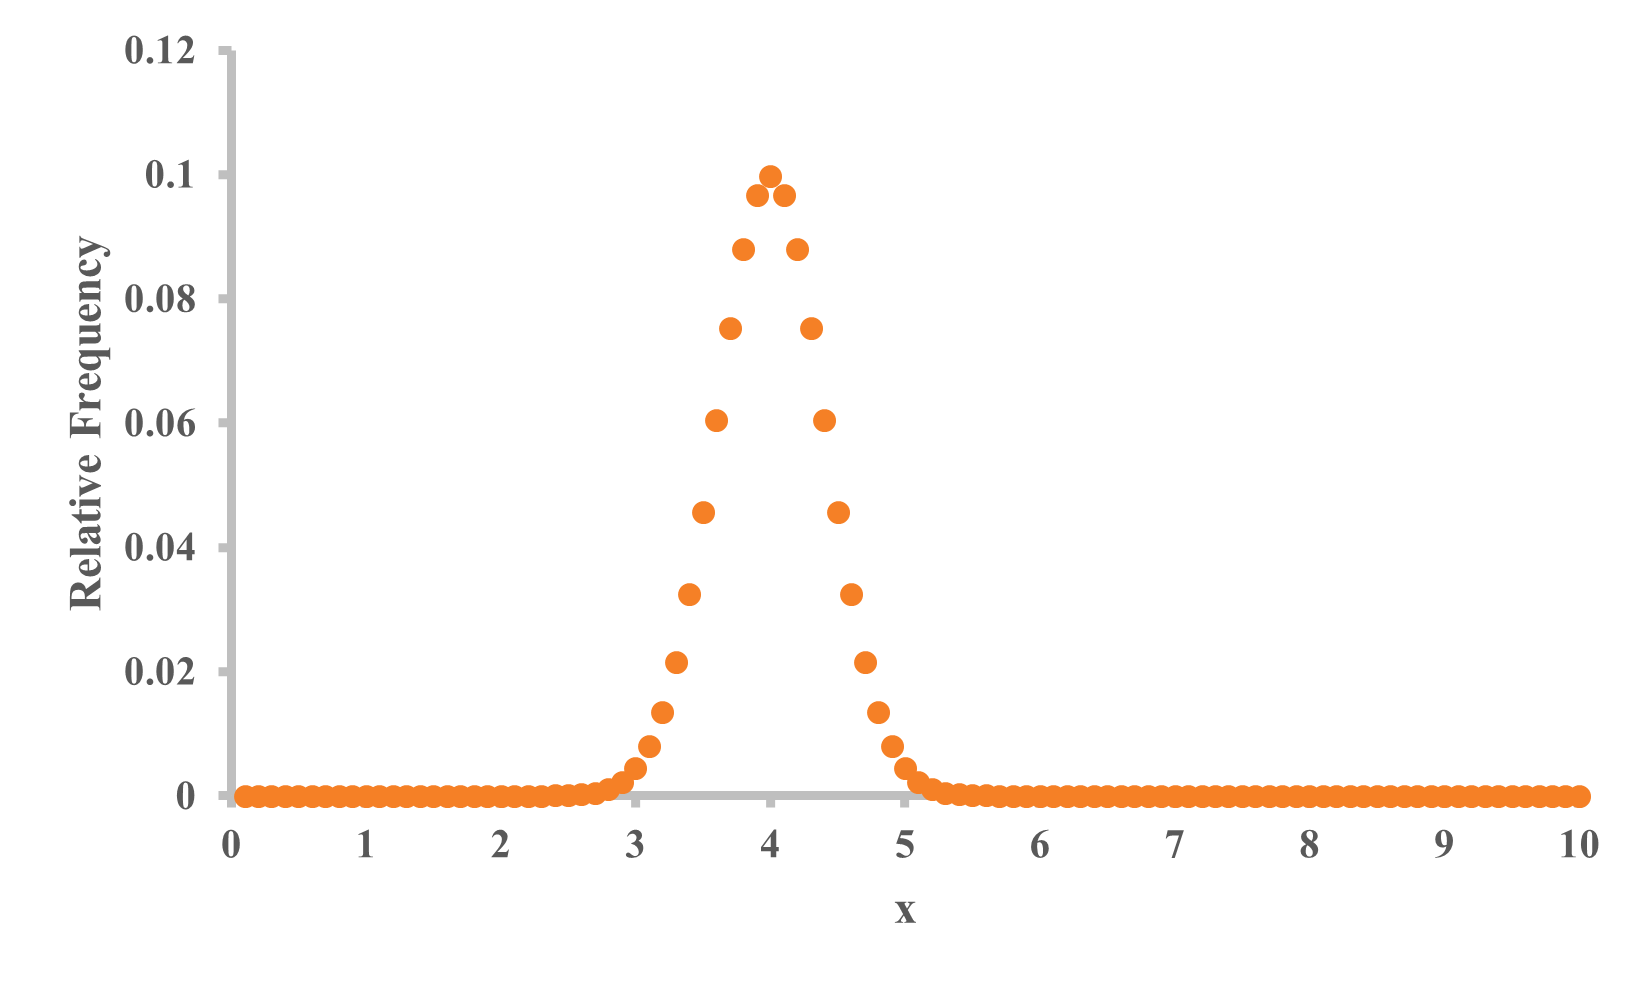
\includegraphics[width=\textwidth]{graphs/DistE_Rel.png}
        \caption{Relative Frequency vs.\ \(x\)}
    \end{subfigure}
    \hfill
    \begin{subfigure}[b]{0.45\textwidth}
        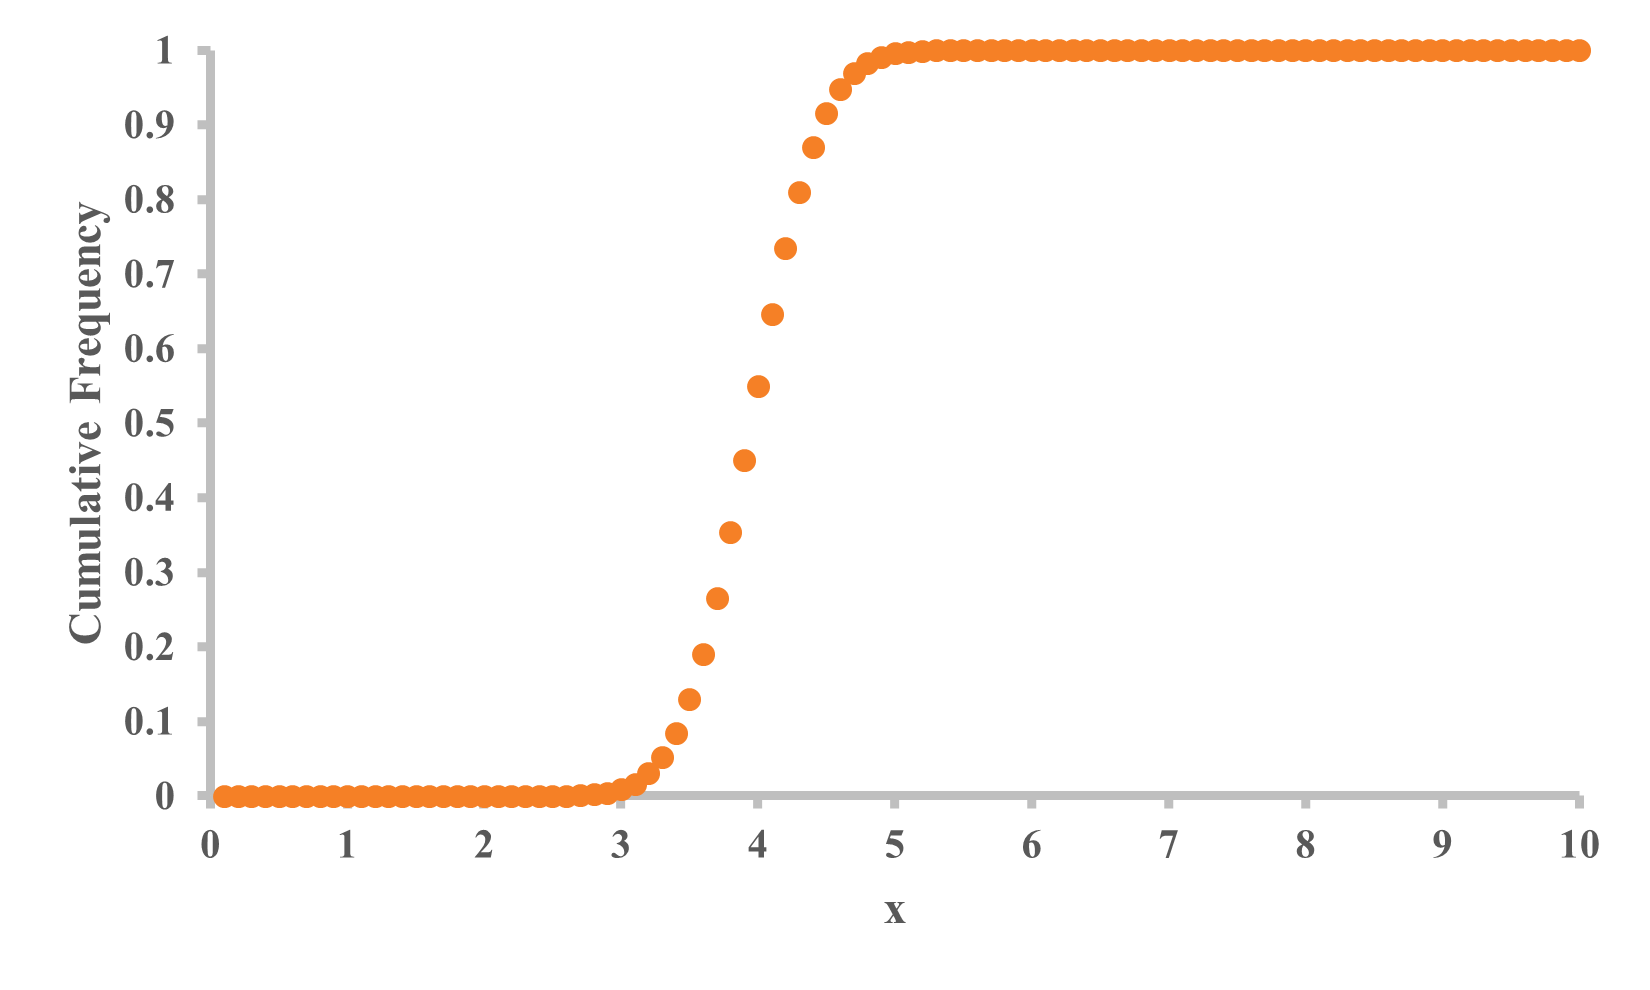
\includegraphics[width=\textwidth]{graphs/DistE_Cumul.png}
        \caption{Cumulative Frequency vs.\ \(x\)}
    \end{subfigure}
    \label{fig:distE}
    \caption{Distribution E}
\end{figure}

\end{document}